%\documentclass{tlp}
%\documentclass[runningheads]{llncs}
\documentclass{llncs}


% Language setting
% Replace `english' with e.g. `spanish' to change the document language
% \usepackage[english]{babel}

% Set page size and margins
% Replace `letterpaper' with `a4paper' for UK/EU standard size
%\usepackage[letterpaper,top=2cm,bottom=2cm,left=3cm,right=3cm,marginparwidth=1.75cm]{geometry}

% Useful packages
\usepackage{amsmath}
\usepackage{tikz}
\usetikzlibrary{trees}
\usetikzlibrary{positioning} 
\usetikzlibrary{arrows}
\usetikzlibrary{decorations.pathmorphing}
\usetikzlibrary{shapes.multipart}
\usetikzlibrary{shapes.geometric}
\usetikzlibrary{calc}
\usetikzlibrary{positioning} 
\usetikzlibrary{fit}
\usetikzlibrary{backgrounds}
\usetikzlibrary{automata}
\usepgflibrary{shapes.geometric}
\usetikzlibrary{shapes.geometric}
\usepackage{mathpartir}
\usepackage{listings}
\usepackage{proof}
\newtheorem{theorem}{Theorem}
\newtheorem{lemma}{Lemma}

\usepackage{graphicx}
%\usepackage[colorlinks=true, allcolors=blue]{hyperref}


\lstdefinelanguage{L4}
{morekeywords={
      assert 
    , class  
    , decl   
    , defn   
    , extends
    , lexicon
    , fact   
    , rule   
    , derivable
    , let   
    , in    
    , not   
    , forall
    , exists
    , if   
    , then 
    , else 
    , for  
    , true 
    , false
},    
sensitive=false,
morecomment=[l]{\#},
morestring=[b]",
}

\lstset{frame=tb,
  language=L4,
  aboveskip=3mm,
  belowskip=3mm,
  showstringspaces=false,
  columns=flexible,
  basicstyle={\footnotesize\ttfamily},
  numbers=none,
  numberstyle=\tiny\color{gray},
  keywordstyle=\color{blue},
  commentstyle=\color{green},
  stringstyle=\color{mauve},
  breaklines=true,
  breakatwhitespace=true,
  tabsize=2
}

%%% Local Variables: 
%%% mode: latex
%%% TeX-master: "main"
%%% End: 

% Theorems and definitions

% \newtheorem{definition}{Definition}
% \newtheorem{theorem}{Theorem}
% \newtheorem{lemma}{Lemma}
% \newtheorem{proposition}{Proposition}


% Definition of colors
\newcommand{\blue}[1]{{\color{blue}#1}}
\newcommand{\green}[1]{{\color{green}#1}}
\newcommand{\red}[1]{{\color{red}#1}}
\newcommand{\gray}[1]{{\color{gray}#1}}

% From MSCS file
\newcommand{\eg}{\textit{e.g.\ }}
\newcommand{\etal}{\textit{et al.\ }}
\newcommand{\etc}{\textit{etc}}
\newcommand{\ie}{\textit{i.e. }}
\newcommand{\viz}{\textit{viz.\ }}
\newcommand{\wrt}{\textit{w.r.t.\ }}
\newcommand{\lex}{\langle}
\newcommand{\rex}{\rangle}

% Own abbreviations
\newcommand{\secref}[1]{Section~\ref{#1}}
\newcommand{\secrefs}[1]{Sections~\ref{#1}}
\newcommand{\figref}[1]{Figure~\ref{#1}}
\newcommand{\figrefs}[1]{Figures~\ref{#1}}
\newcommand{\pgref}[1]{page~\pageref{#1}}
\newcommand{\theoremref}[1]{Theorem~\ref{#1}}
\newcommand{\theoremrefs}[1]{Theorems~\ref{#1}}
\newcommand{\lemmaref}[1]{Lemma~\ref{#1}}
\newcommand{\exampleref}[1]{Example~\ref{#1}}
\newcommand{\defref}[1]{Definition~\ref{#1}}

\newcommand{\figline}{\rule{\textwidth}{0.5pt}}


% Logique

\newcommand{\IMPL}[0]{\longrightarrow}
\newcommand{\IMPLL}[0]{\Longrightarrow} % another implication, to make
                                % a difference with reduction relations
\newcommand{\AND}[0]{\land}
\newcommand{\OR}[0]{\lor}
\newcommand{\NOT}[0]{\lnot}
\newcommand{\FALSE}[0]{\perp}
\newcommand{\TRUE}[0]{\top}
\newcommand{\IFF}[0]{\leftrightarrow}
\newcommand{\BIGAND}[1]{\bigwedge_{#1}}
\newcommand{\BIGOR}[1]{\bigvee_{#1}}
\newcommand{\BIGANDC}[2]{\bigwedge_{#1|#2}} % bigand with constraint
\newcommand{\BIGORC}[2]{\bigvee_{#1|#2}}    % bigor with constraint

\newcommand{\exgeq}[1]{\exists^{{\geq #1}}}
\newcommand{\exeq}[1]{\exists^{{= #1}}}
\newcommand{\exle}[1]{\exists^{{< #1}}}

% Remark macros for the authors

\newcommand{\remms}[2][]{\todo[color=green!40,#1]{MS: #2}}
\newcommand{\remre}[2][]{\todo[color=blue!40,#1]{RE: #2}}
\newcommand{\remjhb}[2][]{\todo[color=blue!20,#1]{JHB: #2}}


% Other

\newcommand{\smalltalcq}[0]{{\small small}-t{$\cal ALCQ$}}
\newcommand{\smalltalcqe}[0]{{\small small}-t{$\cal ALCQ$e}}
\newcommand{\trule}[0]{\xhookrightarrow}
\newcommand{\tableaurule}[1]{{\xhookrightarrow[]{#1}}}
\newcommand{\nodes}[1]{{\cal N}({#1})}
\newcommand{\trans}[1]{{\cal T}({#1})}
\newcommand{\transm}[1]{{\cal T'}({#1})}
\newcommand{\rconts}[1]{\llparenthesis #1 \rrparenthesis} %record contents
\newcommand{\rupd}[2]{{#1}\llparenthesis #2 \rrparenthesis} %record update

\newcommand{\eform}[0]{\mathit{eform}}
\newcommand{\form}[0]{\mathit{form}}
\newcommand{\free}[0]{\mathit{free}}
\newcommand{\exclprop}[0]{\stackrel{\times}{\longrightarrow}}

%%% Local Variables: 
%%% mode: latex
%%% TeX-master: "main"
%%% End: 

\usepackage[colorlinks,hyperindex,bookmarks,linkcolor=blue,citecolor=blue,urlcolor=blue]{hyperref}

%\usepackage[authoryear]{natbib}

\begin{document}

% \lefttitle{Lim, Mahajan, Strecker, Wong}

% \jnlPage{1}{8}
% \jnlDoiYr{2021}
% \doival{10.1017/xxxxx}

\title{Compliance through Model Checking}

\author{
Avishkar Mahajan\orcidID{0000-0002-9925-1533} \and
Martin Strecker\thanks{part of the work carried out at Toulouse University}
\orcidID{0000-0001-9953-9871}\and
Watt Seng Joe\orcidID{0000-0002-6883-4736} \and
Meng Weng Wong\orcidID{0000-0003-0419-9443}
}
\institute{Singapore Management University}
%\authorrunning{Lim, Mahajan, Strecker, Wong}
\authorrunning{Mahajan \and Strecker \and Watt \and Wong}

% \history{\sub{xx xx xxxx;} \rev{xx xx xxxx;} \acc{xx xx xxxx}}

\maketitle

\begin{abstract}
\begin{abstract}
The abstract
\end{abstract}  


%%% Local Variables:
%%% mode: latex
%%% TeX-master: "main.tex"
%%% End:

\end{abstract}

\keywords{
  Compliance,
  Knowledge representation and reasoning,
  Computational Law,
  Model Checking
}


%----------------------------------------------------------------------

\section{Introduction}\label{sec:introduction}

The goal of this paper is to show how a bottom up ASP reasoner like Clingo can be used for Abductive reasoning over First Order Horn clauses. As mentioned in the abstract previous work in abductive reasoning has mostly focused on implementing abduction in a top-down manner with Prolog as the underlying engine. CIFF \cite{mancarella09:_ciff} is a prominent example of this. More recently sCASP \cite{arias19:_const_answer_set_progr_groun_applic,arias_phd_2019} has been developed as a goal directed ASP implementation that can be used for abduction but this too uses a top down method for query evaluation. However there may be use cases where one wants to know all the resulting consequences of an abductive solution to a query with respect to a rule-set. Also, as mentioned in the abstract, top-down methods can sometimes result in solvers that are not truly declarative. Therefore an abductive reasoner that uses a solver like Clingo \cite{gebser12:_answer_set_solvin_pract} can
complement the abilities of goal directed reasoners like sCASP, CIFF \etc.

This paper shows how, given an input ASP rule set, one can write a new ASP program based on that rule set which will yield abductive solutions to queries, with the input ASP rule set as the background theory. The user does not have to explicitly specify the space of abducibles. This translation from the input ASP rule set to the derived ASP program is a purely mechanical one. The key idea is to encode backward chaining over the input rules through the use of meta predicates which incorporate a notion of 'reversing' the input rules to recursively generate pre-conditions from post conditions thereby generating a maximal space of abducibles. Then having generated this maximal space of abducibles, this 'feeds into' another part of the program where we have a representation of the input rules in the normal 'forward' direction. Entailment of the specified query is then checked via an integrity constraint and a minimal set of abduced facts is returned.

The main technical challenges are dealing with situations where input rules have existential variables in pre-conditions or when the query itself has existential variables. The other challenge is to control the depth of the abducibles generation process. The work that seems to come closest to ours is \cite{schueller16:_model_variat_first_order_horn}. It too uses some similar meta predicates to encode backward chaining, and a forward representation of the rules to check for query entailment via integrity constraints.

However there are several novel features in our work.  Firstly, depth  control for abducible generation is done in a purely declarative way as part of the encoding itself without needing to call external functions or other pieces of software. Furthermore, adding facts to the program automatically gives an implicit form of term substitution where Skolem terms or
other 'place-holder' terms occurring in abducibles are replaced away so that
the resulting proof is simplified, without any need for an explicit representation of equality between terms. Past work on this topic such as \cite{schueller16:_model_variat_first_order_horn} models equality between terms via an explicit equality predicate which may become unwieldy. Another approach to dealing with existential variables encountered during the abductive proof search is to simply ground all the rules over the entire domain of constants. However, this can often lead to too many choices for what an existential variable may be substituted for which may result in unexpected/unintuitive solutions. Our method avoids both of these techniques. We present three main sets of abductive proof generation encodings. One of the encodings only supports partial term substitution whereas the other two support full term substitution. Lastly, we also present an encoding which generates a set of directed edges representing a justification 
graph  for the generated proof, where the graph can be of any desired depth.

The rest of the paper is organised as
follows. First we give a brief introduction to Answer Set Programming and Abductive reasoning then, Section~\ref{sec:abductive_proof} defines the problem being tackled more formally. Section~\ref{sec:derived_asp} presents the encodings that facilitate the abductive proof generation and directed edge generation. The sections that follow discuss some formal results regarding completeness, finiteness of abductive proof generation. We also discuss a formal result regarding term substitution. Finally Section~\ref{sec:conclusion} discusses
future work and concludes.

This is an extended version of a paper presented at PPDP~2022 \cite{ppdp_version}.

\subsection{Answer Set Programming}
Answer Set Programming (ASP) is a declarative language from the logic programming family. It is widely used and studied by knowledge representation and reasoning and symbolic AI researchers for its ability to model common sense reasoning, model combinatorial search problems etc. It incorporates the $\textit{negation-as-failure}$ operator as interpreted under the $\textit{stable model semantics}$. Clingo is a well established implementation of ASP, incorporating additional features such as $\textit{choice rules}$ and optimization statements. We shall only briefly touch upon various aspects of ASP and Clingo here. The reader may consult \cite{gebser12:_answer_set_solvin_pract} for a more thorough description. Each rule in an ASP program consists of a set of body atoms. Some of these body atoms maybe negated via the negation as failure operator $not$. Rules with no pre-conditions are called facts. Given a set of rules $R$ and a set of facts $F$, the Clingo solver computes all stable models of the ASP program $F\cup R$. For example given the fact $r(alpha)$ and the rules:
\begin{lstlisting}[frame=none]
p(X):-r(X),not q(X).
q(X):-r(X), not p(X).
\end{lstlisting}
The solver will show us 2 models or answer sets given by\\ $\{r(alpha),p(alpha)\}$ and $\{r(alpha),q(alpha)\}$. Note that as opposed to Prolog, Clingo is a bottom up solver meaning that it computes complete stable models (also known as answer sets) given any ASP program. An integrity constraint is formally speaking a rule whose post-condition is the boolean $false$. In ASP, integrity constraints are written as rules with no post-conditions and are used to eliminate some computed answer sets. For example given in the following ASP program
\begin{lstlisting}[frame=none]
r(alpha).
p(X):-r(X),not q(X).
q(X):-r(X), not p(X).
:-q(X).
\end{lstlisting}
any answer set where some instantiation of $q$ is true is eliminated. Hence we get just one answer set. $\{r(alpha),p(alpha)\}$.\\ We will now give a quick introduction to two features of Clingo that we will use throughout this paper. Namely $\textit{choice rules}$ and $\textit{weak constraints}$. Weak constraints are also often known as optimization statements. Intuitively a choice rule is a rule where if the pre-conditions are satisfied then the post-condition may or may not be made true. The post-condition of a choice rule is enclosed in curly brackets. So given the following ASP program:\begin{lstlisting}[frame=none]
r(alpha).
{q(X)}:-r(X).
\end{lstlisting}, where the rule is a choice rule the solver will give us 2 models namely $\{r(alpha)\}$, $\{r(alpha),q(alpha)\}$. If we modify the program by adding an integrity constraint like so:
\begin{lstlisting}[frame=none]
r(alpha).
{q(X)}:-r(X).
:-q(X).
\end{lstlisting}
then we get just one model $\{r(alpha)\}$.\\
Weak constraints are used in Clingo to order answer sets by preference according to the atoms that appear in them. Without going into too much detail let us just explain the meaning of one kind of weak constraint which is the only kind that we will use in the paper namely:
\begin{lstlisting}[frame=none]
:~a(X). [1@1,X]
\end{lstlisting}
Adding this to an ASP program, orders the answer sets of the program according to the number of distinct instantiations of the predicate $a$ in the answer set. The answer set with the least number of instantiations of $a$ is called the most $optimal$ answer set. 
\subsection{Abductive Reasoning}
Briefly, abduction is a reasoning process where given a background theory $T$, we wish to find a set of facts $F$ such that $F\cup T$ is consistent and $F\cup T$ entails some goal $g$ for some given entailment relation. Usually we also want $F$ to be minimal in some well defined sense. Traditional Abductive Logic Programming has a long history, but we have our own definitions of what it means to formulate and solve an abductive reasoning problem and we will make all the relevant concepts/notions precise in the sections that follow.  


%%% Local Variables:
%%% mode: latex
%%% TeX-master: "main"
%%% End:

% ----------------------------------------------------------------------
\section{Case Study: PDPA}\label{sec:case_study_pdpa}

Singapore's Personal Data Protection Act \cite{pdpa_link} consists of a set of
rules governing the use of personal data in private and public organizations,
and describes actions to be taken if a data breach is detected. It consists on
the one hand of \emph{constitutive} rules, \ie definitions specifying
what is considered a data breach and under which conditions it is deemed a
notifiable data breach. On the other hand, \emph{regulative} rules prescribe
which actions need to be taken if a notifiable data breach is detected.

The constitutive rules are sufficiently voluminous and complex to warrant the
development of an expert system assisting organizations in assessing whether a
data breach is notifiable. In the CCLAW project, we have developed such a
system. The regulative rules
are seemingly less involved but sufficiently intricate that actors that
precisely follow the rules may wind up in a state where they have breached the
law. The complexity results from the interplay of temporal conditions that
remain implicit and that would have to be explicated to guarantee lawful
behavior.

We here give an abridged account of the relevant rules; for details, see
\S\S~26A to E of \cite{pdpa_link} that leads to and motivates our
formalization in \secref{sec:formal_analysis}. The PDPA identifies three
actors in a data breach scenario:
\begin{itemize}
\item the \emph{organization} in which a data breach has occurred;
\item the Personal Data Protection Commission (PDPC, henceforth only called
  the \emph{commission}), the governmental authority that has to be notified
  in case of a breach;
\item the \emph{individual} affected by a data breach. The abstraction of the
  multitude of affected individuals to a single entity is already done in the
  law text and seems appropriate as there is no interaction among the
  individuals. 
\end{itemize}

The temporal requirements are as follows:
\begin{itemize}
\item When a data breach is detected, the organization has up to thirty days to
  assess whether the data breach is notifiable; if it is not, no further
  action is required, and the process stops there. 
\item If the breach is notifiable, the organization is obliged to inform the
  commission within three days of having recognized the breach as notifiable.
\item If the breach is notifiable, any affected individual also has to be
  informed within the three day period.
\item The organization must not notify an affected individual if the
  commission so directs.
\end{itemize}

The inconsistency, that was in part revealed by the formalization and then
confirmed by model checking, arises from the lack of temporal coordination
between the action of informing the commission and the individual, and
possibly the interdiction by the commission to inform the individual.


%----------------------------------------------------------------------
\section{Formal Analysis}\label{sec:formal_analysis}

%......................................................................
\subsection{Formal Model}\label{sec:formal_model}

We have carried out a formal analysis of this scenario with Timed Automata
(TA) in the Uppaal \cite{larsen1997uppaal} model checker. The global setup is
shown in \figref{fig:pdpa}. There are three interacting automata, one for each
of the above-mentioned actors. The states carry names (in mauve), the initial
states are marked with a double circle. The automata synchronize via messages
(in turquoise), where a send action is indicated by an exclamation and a
receive action by a question mark. Transitions may depend on Boolean
conditions (here: variables such as \texttt{isNotifiable}) and on temporal
conditions modeled with the aid of \emph{clocks}. In this example, there is
one clock, \texttt{cl}, that is zero in the initial state, and that is again
reset to zero in the transition from the state \texttt{breachDetected} to
\texttt{breachDeterminedNotifiable}.


\begin{figure}[htp]
\centering
\subfloat[Commission\label{fig:commission}]{%
  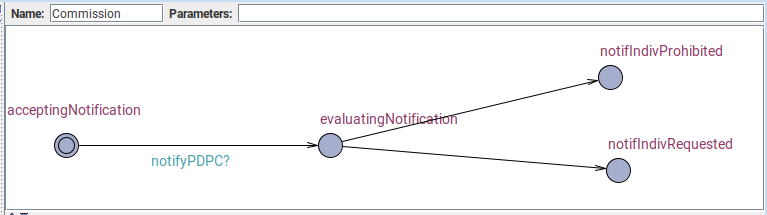
\includegraphics[width=0.65\textwidth]{Figures/commission.png}%
}\hfil
\subfloat[Individual\label{fig:individual}]{%
  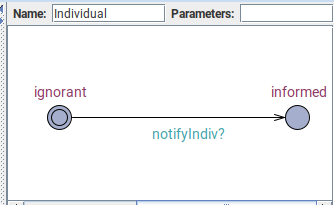
\includegraphics[width=0.3\textwidth]{Figures/individual.png}%
}\\
\subfloat[Organization\label{fig:organization}]{%
  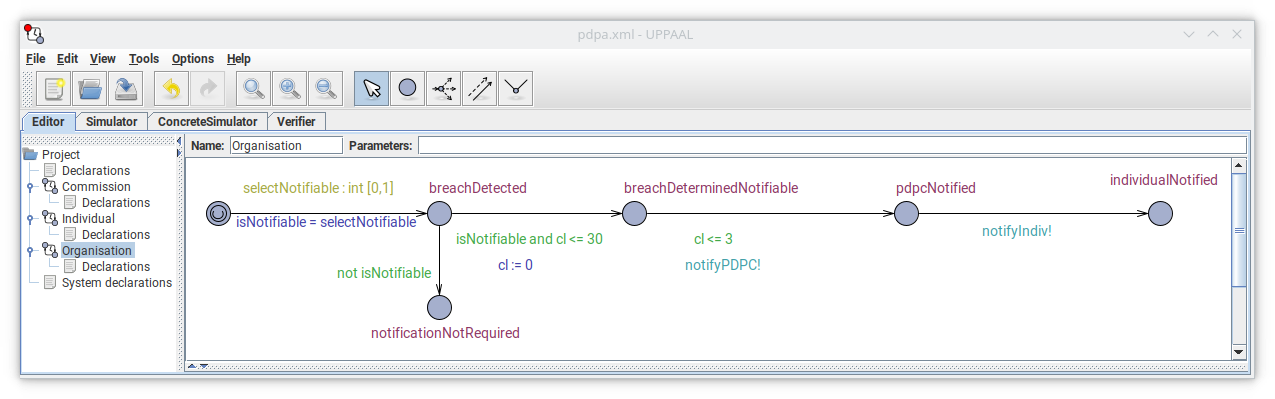
\includegraphics[width=\textwidth]{Figures/organization.png}%
}
\caption{Automata modeling the PDPA scenario}\label{fig:pdpa}
\end{figure}

According to the TA semantics, there are two kinds of transitions: the passage
of time, at the same rate in all automata, or discrete state changes along
enabled transitions, \ie transitions whose conditions are satisfied. In case
several transitions are enabled, one of them is chosen
non-deterministically. This happens for example in the Commission automaton
after receiving a notification (\texttt{notifyPDPC?}), modeling the fact that
the commission's decision to prohibit or request the notification of the
affected individual is autonomous and not influenced by external factors.
The Individual automaton only provides two states corresponding to whether the
individual has not yet / has been notified.

The Organization automaton is the
most complex one: the very first transition is a modeling artifact for giving
a random Boolean value to the variable \texttt{isNotifiable}. If the data
breach is not notifiable, the process ends. If the breach is determined to be
notifiable within 30 days, the timer is reset to allow for a 3 day period before
the notification is carried out. We have here made the choice to sequentialize
the notifications (the commission, then the individual). An interleaved execution
would be preferable but is hampered by limitations of Uppaal (no nested
parallel automata).

Let us note that our automaton model is not complete: not every execution of
the automata will run to completion, \ie wind up in one of the end nodes of
the automata. Instead, an execution can get stuck in an intermediate
state. This choice is deliberate, but open to debate: adding failure states
for every undesirable run would clutter up the automata; some runs may
legitimately be infinite without clearly identified end states; and, as seen
below, such deadlock states can be detected.

%......................................................................
\subsection{Checking the Model}\label{sec:checking_the_model}

The model can be validated in several respects. The simplest form corresponds
to testing in traditional program development. For this, Uppaal (and similar
tools) provides a \emph{simulation} environment whose purpose is to step
through the model depending on user-selected criteria, for example the values
of Boolean variables or the duration of staying in particular system
states. We will not further dwell on simulation, also because error traces
(see below) can be run in the simulator.

Contrasting with simulation is a systematic state space exploration by model
checking. Model checking can be used in legal drafting mode, to discover
incoherences in a law. It can also be used in ``production'' mode to identify
illegal behaviors and possible contrary-to-duty repair actions. We will
present examples of the two kinds below.

\begin{figure}[htp]
\centering
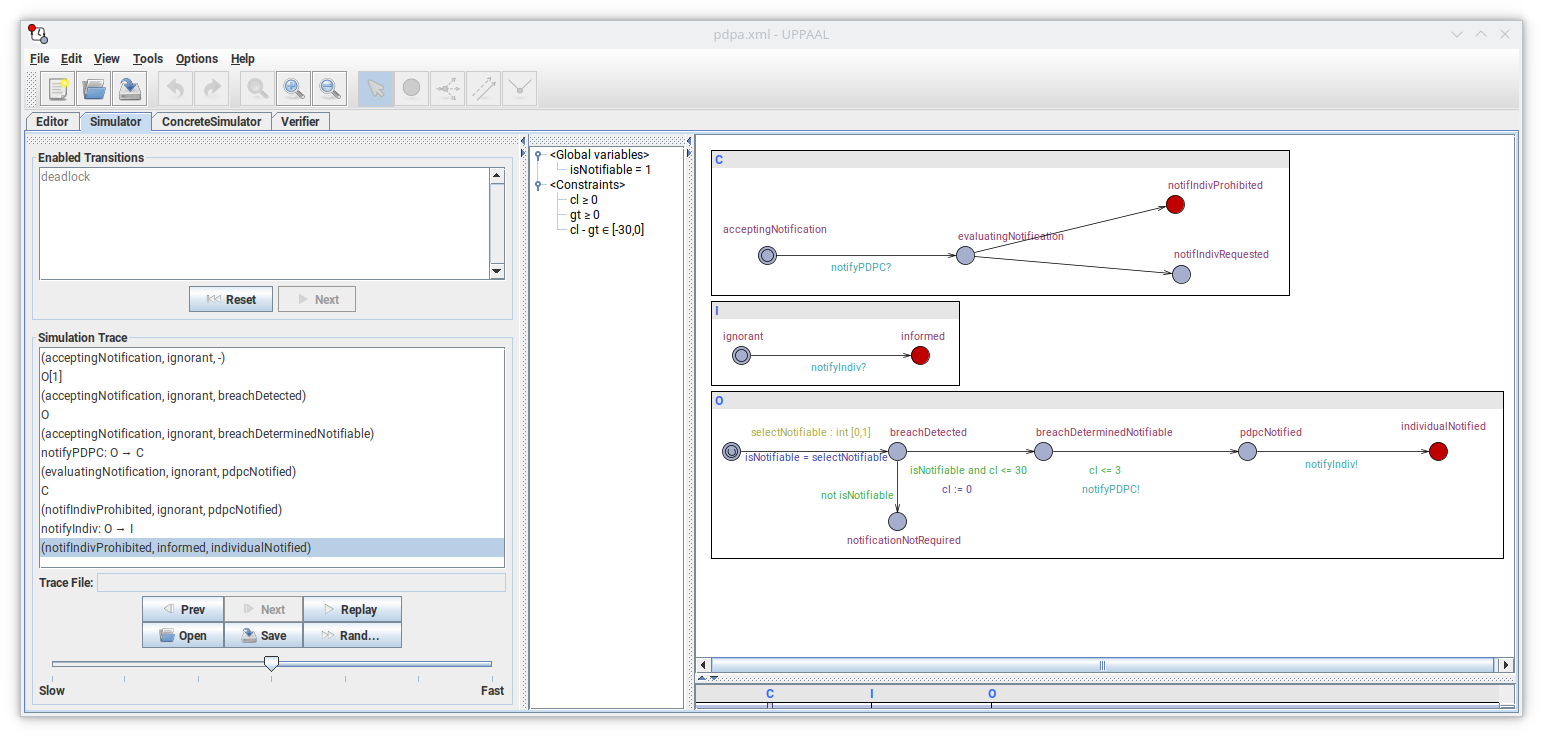
\includegraphics[width=\textwidth]{Figures/pdpa_trace.png}
\caption{Failure trace}\label{fig:pdpa_trace}
\end{figure}

Model checking tries to verify if a system's behavior conforms to requirements
that are typically stated in a formal logic, here the temporal logic CTL. We
give a few  examples in our scenario:

\begin{itemize}
\item A desirable property is that it is possible to reach a state such that the
  individual is informed and the commission requests informing the
  individual. This property is written as
  \begin{alltt}E<>I.informed and C.notifIndivRequested \end{alltt}
  Here, \texttt{E<>} means: ``there exists a run
  eventually leading to''. and \texttt{I.informed} and
  \texttt{C.notifIndivRequested} refer to the corresponding states in the
  Individual and Commission automata. This property is indeed satisfied.

  
\item An undesirable situation is that the individual is informed in spite of
  the commission having prohibited it, expressed by the formula
  \begin{alltt}E<> I.informed and C.notifIndivProhibited\end{alltt}. This property is also satisfied,
  and Uppaal produces a trace (\figref{fig:pdpa_trace}) leading to this error
  situation. It comes about because the organization has no clue at which
  point the commission's interdiction to inform the individual could
  intervene, and is therefore entitled to inform the individual as soon as a
  data breach is identified.

\item Another undesirable behavior is when the execution of the process gets
  stuck, or, more precisely, when there is a deadlock, in a system state that
  is not perceived as final. Note that in a technical sense, according to the
  terminology of labelled transition systems, every system with final states
  is deadlocked in these states. Identifying deadlocks in ``intermediate''
  states may contribute to finding leaks in the formal model, or states that
  correspond to breaches of the law. For example, the intermediate state
  \texttt{breachDeterminedNotifiable} is identified by the query
  \begin{alltt}E<> O.breachDeterminedNotifiable and deadlock\end{alltt}
  as a deadlock state. Indeed, in
  this state, no action is possible when the notification deadline of 3 days
  has been exceeded.
\end{itemize}

% \begin{tabular}{ll}
% (acceptingNotification, ignorant, \emph{initial}) & O \\
% (acceptingNotification, ignorant, breachDetected) & O \\
% (acceptingNotification, ignorant, breachDeterminedNotifiable) & C, O\\
% (evaluatingNotification, ignorant, pdpcNotified) & C \\
% (notifIndivProhibited, ignorant, pdpcNotified) & I, O\\
% (notifIndivProhibited, informed, individualNotified) & \\
% \end{tabular}


%----------------------------------------------------------------------
\section{Discussion: Extensions and Refinements}\label{sec:discussion}


%......................................................................
\subsection{Refining the Model}\label{sec:refining_model}

The formal model could be perceived as ``incomplete'' in several respects. As
shown by the formal analysis of \secref{sec:formal_analysis}, some behaviors
are \emph{undefined} (and lead to deadlocks), others are
\emph{under-specified}. In particular, a precise interaction between the
commission and the organization is not made explicit in the law text, which
might question the tenet of ``isomorphism''
\cite{bench_capon_gordon_isomorphism_2009} between law texts and formal
representations: the formal representation possibly has to make completions to
avoid undesirable situations.

One such completion would be the following: the commission communicates its
decision back to the organization before the organization informs the
individual. Such a provision is currently not foreseen in the law text. In
order for the deadline of informing the individual (call it $d_i$) to be
satisfied, the commission's response (call it $d_c$) would have to arrive
before: $d_c < d_i$. These additional constraints can be incorporated into the
automaton model and would avoid the above error scenario.


%......................................................................
\subsection{Realizability}\label{sec:realizability}

Laws are requirements that constrain processes adopted by companies and
organizations and that are often described by business processes
\cite{aalst_business_provess_management_comprehensive_survey_2013}.

We take an automaton such as in \figref{fig:organization} as an abstract
specification of a business process. Depending on an organization's internal
functioning, such an abstract description will be further refined, typically
by adding new states (for example to guide the investigations to determine if
a breach is notifiable). We will then have two automata, the abstract one
(such as in \figref{fig:organization}) and its refinement (the business
process, possibly specified in a dedicated language such as BPMN). Since tools such
as Uppaal do not offer support for refinement checking, our project currently
works on a language for describing refinements and for verifying them.

Of particular interest for the legal drafter in this context is the question
of \emph{realizability}: can laws be implemented under realistic conditions?
To continue the example of \secref{sec:refining_model}: formally, the
requirement $d_c < d_i$ on the deadlines is not a sufficient guarantee for
realizability under realistic conditions: the difference $d_i - d_c$ can
become arbitrarily small. Detecting such inconsistencies is part of our
ongoing work.

%......................................................................
\subsection{Modularization through Rely-Guarantee Reasoning}\label{sec:rely_guarantee}

The previous discussion highlights another desideratum: modularization. The
organization can only satisfy requirements imposed on them when other actors
(such as the commission) satisfy theirs. For separate refinement (in the sense
of \secref{sec:realizability}) to work, an (abstract) automaton should be
annotated with requirements it expects its environment to provide (the
\emph{rely} part of its specification) in order to deliver the promise it
makes about its behavior (the \emph{guarantee} of the specification). 

Without having clearly identified solutions, we are interested in exploring
the duality of notions such as permissions (and \emph{reliance} statements in
a specification) and obligations (\emph{guarantees}) known from deontic
logics, notions that have been largely explored, among others, in LogiKEy
\cite{benzmueller_etal_logikey_2020}. 

A whole line of work is concerned with formal contracts
\cite{benveniste_raclet_etal_ContractsMonograph2018}, and in particular
notions of modularization and refinement
\cite{Alfaro2005,grumberg_lang_model_checking_modular_verification_2004}. In a
legal context, similar ideas have in particular been proposed as a temporal
logic of normative systems
\cite{agotnes_hoek_aguilar_sierra_woolridge_temporal_logic_normative_systems_2009}. 

%%% Local Variables:
%%% mode: latex
%%% TeX-master: "main"
%%% End:




%\subsection*{Acknowledgements}
\paragraph{Acknowledgements.}
This research / project is supported by the National Research Foundation,
Singapore under its Industry Alignment Fund – Pre-positioning (IAF-PP) Funding
Initiative. Any opinions, findings and conclusions or recommendations
expressed in this material are those of the author(s) and do not reflect the
views of National Research Foundation, Singapore.

%----------------------------------------------------------------------
% \bibliographystyle{tlplike}
\bibliographystyle{splncs04}
\bibliography{main}

%----------------------------------------------------------------------
% \newpage
% \appendix
% \section{An Overview of the L4 Language: Details}\label{sec:l4_language_app}

Let us give some more details about the L4 language: its class and type
definition mechanism, and the way it handles proof obligations.
\remms[inline]{Integrate l4\_language.tex}

% ----------------------------------------------------------------------
\subsection{Terminology and Class Definitions}\label{sec:classdefs}

The definition in \figref{fig:classdefs} introduces classes for vehicles, days
and roads. 

\begin{figure}[h!]
%\begin{mdframed}
\begin{lstlisting}
class Vehicle {
   weight: Integer
}
class Car extends Vehicle {
   doors: Integer
}
class Truck extends Vehicle
class SportsCar extends Car

class Day
class Workday extends Day
class Holiday extends Day

class Road
class Highway extends Road
\end{lstlisting}
%\end{mdframed}
  \caption{Class definitions of speedlimit example}\label{fig:classdefs}
\end{figure}

Classes are arranged in a tree-shaped hierarchy, having a class named
\texttt{Class} as its top element. Classes that are not explicitly derived
from another class via \texttt{extends} are implicitly derived from
\texttt{Class}. A class $S$ derived from a class $C$ by \texttt{extends} will
be called a subclass of $C$, and the immediate subclasses of \texttt{Class}
will be called \emph{sorts} in the following. Intuitively, classes are meant
to be sets of entitities, with subclasses being interpreted as
subsets. Different subclasses of a class are not meant to be disjoint.

Class definitions can come with attributes, in braces. These attributes can be
of simple type, as in the given example, or of higher type (the notion of type
will be explained in \secref {sec:fundecls}). In a declarative reading,
attributes can be understood as a shorthand for function declarations that
have the class they are defined in as additional domain. Thus, the attribute
\texttt{weight} corresponds to a top-level declaration \texttt{weight: Vehicle
  -> Integer}. In a more operational reading, L4 classes can be understood as
prototypes of classes in object-oriented programming languages, and an
alternative field selection syntax can be used: For \texttt{v: Vehicle}, the
expression \texttt{v.weight} is equivalent to \texttt{weight(v)}, at least
logically, even though the operational interpretations may differ.


% ----------------------------------------------------------------------
\subsection{Types and Function Declarations}\label{sec:fundecls}

L4 is an \emph{explicitly} and \emph{strongly typed} language: all entities
such as functions, predicates and variables have to be declared before being
used. One purpose of this measure is to ensure that the executable sublanguage
of L4, based on the simply-typed lambda calculus with subtyping, enjoys a type
soundness property: evaluation of a function cannot produce a dynamic type
error.

\figref{fig:fundecls} shows two function declarations. Functions with
\texttt{Boolean} result type will sometimes be called \emph{predicates} in the
following, even though there is no syntactic difference. All the declared
classes are considered as elementary types, as well as \texttt{Integer},
\texttt{Float}, \texttt{String} and \texttt{Boolean} (which are internally also treated as
classes). If $T_1, T_2, \dots T_n$ are types, then so are function types
\texttt{$T_1$ -> $T_2$} and tuple types \texttt{($T_1$, $\dots$ ,$T_n$)}. The
type system and the expression language, to be presented later, are
higher-order, but extraction to some solvers will be limited to
(restricted) first-order theories.

\begin{figure}[h]
%\begin{mdframed}
\begin{lstlisting}
decl isCar : Vehicle -> Boolean
decl maxSp : Vehicle -> Day -> Road -> Integer -> Boolean
\end{lstlisting}
%\end{mdframed}
  \caption{Declarations of speedlimit example}\label{fig:fundecls}
\end{figure}

The nexus between the terminological and the logical level is established with
the aid of \emph{characteristic predicates}. Each class $C$ which is a
subclass of sort $S$ gives rise to a declaration \texttt{is$C$: $S$ ->
  Boolean}. An example is the declaration of \texttt{isCar} in
\figref{fig:fundecls}. In the L4 system, this declaration, as well as the
corresponding class inclusion axiom, are generated
automatically.

Two classes derived from the same base class (thus: \texttt{$C_1$ extends $B$}
and \texttt{$C_2$ extends $B$}) are not necessarily disjoint. 

From the subclass relation, a \emph{subtype} relation $\preceq$ can be defined
inductively as follows: if \texttt{$C$ extends $B$}, then $C \preceq B$, and
for types $T_1, \dots, T_n, T_1', \dots, T_n'$,
if $T_1 \preceq T_1', \dots, T_n \preceq T_n'$, 
then \texttt{$T_1'$ -> $T_2 \; \preceq \; T_1$ -> $T_2'$} 
and \texttt{($T_1$, $\dots$, $T_n$) $\preceq$ ($T_1'$, $\dots$, $T_n'$)}.

Without going into details of the type system, let us remark that it has been
designed to be compatible with subtyping: if an element of a type is
acceptable in a given context, then so is an element of a subtype. In
particular,
\begin{itemize}
\item for field selection, if $C'$ is a class having field $f$ of type $T$,
  and $C \preceq C'$, and $c : C$, then field selection is well-typed with $c.f : T$.
\item for function application, if $f: A' \mbox{\texttt{->}} B$ and $a:A$ and
  $A \preceq A'$, then function application is well-typed with $f\; a : B$.
\end{itemize}



% ----------------------------------------------------------------------
\subsection{Assertions}\label{sec:assertions}


Assertions are statements that the L4 system is meant to verify or to
reject -- differently said, they are proof obligations. These assertions are verified
relative to a rule set comprising some or all of the rules and facts stated
before. 


The active rule set used for verification can be configured, by adding rules
to or deleting rules from a default set. Assume the active rule set consists
of $n$ rules whose logical representation is $R_1 \dots R_n$, and assume the
formula of the assertion is $A$. The proof obligation can then be checked for
\begin{itemize}
\item  \emph{satisfiability}: in this case, $R_1 \AND \dots \AND R_n \AND A$
  is checked for satisfiability.
\item \emph{validity}: in this case, $R_1 \AND \dots \AND R_n \IMPL A$ is
  checked for validity.
\end{itemize}
In either case, if the proof fails, a model resp.{} countermodel is produced.
In the given example, the SMT solver checks the validity of the formula and
indeed returns a countermodel that leads to contradictory prescriptions of the
maximal speed: if the vehicle is a car, the day a workday and the road a
highway, the maximal speed can be 90 or 130, depending on the rule applied.


The assertion \texttt{maxSpFunctional} of \figref{fig:assertions} can be considered an essential
consistency requirement and a rule system violating it is inconsistent \wrt{} the intended semantics of \texttt{maxSp}. One
remedial action is to declare one of the rules as default and the other rule
as overrriding it.

After this repair action, \texttt{maxSpFunctional} will be provable (under
additional natural conditions described in \secref{sec:rule_inversion}). We can now
continue to probe other consistency requirements, such as exhaustiveness
stating that a maximal speed is defined for every combination of vehicle:

\begin{lstlisting}
assert <maxSpExhaustive>
   exists sp: Integer. maxSp instVeh instDay instRoad sp
\end{lstlisting}

The intended usage scenario of L4 is that by an interplay of proving
assertions and repairing broken rules, one arrives at a rule set satisfying
general principles of coherence, completeness and other, more elusive
properties such as fairness (at most temporary exclusion from essential
resources or rights).


%%% Local Variables:
%%% mode: latex
%%% TeX-master: "main"
%%% End:

% % ----------------------------------------------------------------------
\section{Reasoning with and about Rules - Motivation}\label{sec:resasoning_with_rules_app}
% ----------------------------------------------------------------------

To illustrate the use of rule modifiers discussed in
\secref{sec:resasoning_with_rules}, we consider a realistic law text,
Singapore's Professional Conduct Rules \S~34
\cite{professional_conduct_rules}. This case study has been investigated in
detail in \cite{morris21:_const_answer_set_progr_tool}. Here is an excerpt of
the rules:

\begin{description}
\item[(1)] A legal practitioner must not accept any executive appointment
  associated with any of the following businesses: 
  \begin{description}
  \item[(a)] any business which detracts from, is incompatible with, or
    derogates from the dignity of, the legal profession;
  \item[(b)] any business which materially interferes with the legal
    practitioner’s primary occupation of practising as a lawyer; (\dots)
  \end{description}
\item[(5)] Despite paragraph (1)(b), but subject to paragraph (1)(a) and (c)
  to (f), a locum solicitor may accept an executive appointment in a business
  entity which does not provide any legal services or law-related services, if
  all of the conditions set out in the Second Schedule are satisfied.
\end{description}

The two main notions developed in the Conduct Rules are which executive appointments a legal
practictioner \emph{may} or \emph{must not} accept under which
circumstances. As there is currently no direct support for deontic logics in
L4, these notions are defined as two predicates \texttt{MayAccept} and
\texttt{MustNotAccept}, with the intended meaning that these two notions are
contradictory, and this is indeed what will be provable after a complete
formalization.

Let us here concentrate on the modifiers \emph{despite} and \emph{subject
  to}. A synonym of ``despite'' that is often used in legal texts is
``notwithstanding'',  and a synonym of
``subject to'' is ``except as provided in'', see \cite{adams_contract_drafting_2004}.

The reading of rule (5) is the following:
\begin{itemize}
\item ``subject to paragraph (1)(a) and (c) to (f)'' means: rule (5) applies
  as far as (1)(a) and (c) to (f) is not established. Differently said, rules
  (1)(a) and (c) to (f) undercut or defeat rule (5).

  One way of explicitating the ``subject to'' clause would be to rewrite (5)
  to: ``Despite paragraph (1)(b), provided the business does not detract from,
  is incompatible with, or derogate from the dignity of, the legal profession;
  and provided that not [clauses (1)(c) to (f)]; then a locum
  sollicitor\footnote{in our class-based terminology, a subclass of legal
    practitioner} may accept an executive appointment.''

\item ``despite paragraph (1)(b)'' expresses that rule (5) overrides rule
  (1)(b). In a similar spirit as the ``subject to'' clause, this can be made
  explicit by introducing a proviso, however not locally in  rule (5), but
  remotely in rule (1)(b).

  One way of explicitating the ``despite'' clause of rule (5) would be to
  rewrite (1)(b) to: ``Provided (5) is not applicable, a legal practitioner
  must not accept any executive appointment associated with any business which
  materially interferes with the legal practitioner’s primary occupation of
  practising as a lawyer.''
\end{itemize}

The astute reader will have remarked that the treatment in both cases is
slightly different, and this is not related to the particular semantics of
\emph{subject to} and \emph{despite}: we can state defeasibility
\begin{itemize}
\item either in the form of (negated) preconditions of rules: ``rule $r_1$ is
  applicable if the preconditions of $r_2$ do not hold'';
\item or in the form of (negated) derivability of the postcondition of rules: ``rule $r_1$ is
  applicable if the postcondition of $r_2$ does not hold''.
\end{itemize}


%%% Local Variables:
%%% mode: latex
%%% TeX-master: "main"
%%% End:

% \section{Rule Transformation Strategies}\label{sec:rule_transformation_strategies}

In \secref{sec:rule_modifiers_in_classical_logic}, we have discussed one
approach for coding defeasibility in a classical, monotonic logic. We will now
present a second approach (\secref{sec:restr_deriv}) that can potentially lead to more compact
preconditions, but that is more complex because it requires a change of the
signature of predicates. It has so far not been implemented. We compare the
two approaches in \secref{sec:comparison}, showing that they produce
essentially the same derivable models.

% ......................................................................
\subsection{Restriction via Derivability}\label{sec:restr_deriv}

We now give an alternative reading of \texttt{restrictSubjectTo} introduced in
\secref{sec:preprocessing}. To
illustrate the point, let us take a look at a simple propositional example.

\begin{example}\label{ex:small_propositional} Take the definitions:
\begin{lstlisting}
rule <r1> if B1 then C1
rule <r2> {subjectTo: r1} if B2 then C2
\end{lstlisting}
\end{example}

Instead of saying: \texttt{r2} corresponds to
\texttt{\blue{if} B2 \&\& not B1 \blue{then} C2} 
as in \secref{sec:restr_precond}, we would now read it as
``if the conclusion of \texttt{r1} cannot be derived'', 
which could be written as
\texttt{\blue{if} B2 \&\& not C1 \blue{then} C2}.
The two main problems with this naive approach are the following:
\begin{itemize}
\item As mentioned in \secref{sec:reasoning_with_rules}, a \emph{subject to}
  restriction is often applied to rules with contradicting conclusions, so in
  the case that \texttt{C1} is \texttt{not C2}, the generated rule would be a
  tautology.
\item In case of the presence of a third rule
\begin{lstlisting}[frame=none]
rule <r3> if B3 then C1
\end{lstlisting}
a derivation of \texttt{C1} from \texttt{B3} would also block the application
of \texttt{r2}, and \texttt{subjectTo: r1} and \texttt{subjectTo: r1, r3}
would be indistinguishable.
\end{itemize}

We now sketch a solution for rule sets whose conclusion is always an atom (and
not a more complex formula).

\begin{enumerate}
\item In a preprocessing stage, all rules are transformed as follows:
  \begin{enumerate}
  \item We assume the existence of classes \texttt{Rulename$_P$}, one for each
    transformable predicate $P$ (see below).
  \item All the predicates $P$
    occurring in the conclusions of rules (called \emph{transformable
      predicates}) are converted into predicates $P^+$ with one additional
    argument of type \texttt{Rulename$_P$}. In the
    example, \texttt{C1$^+$: Rulename$_{C1}$ -> Boolean} and similarly for \texttt{C2}.
  \item The transformable predicates $P$ in conclusions of rules receive one
    more argument, which is the name \emph{rn} of the rule: $P$ is transformed
    into $P^+\; rn$. The informal reading is ``the predicate is derivable with
    rule \emph{rn}''.
  \item All transformable predicates in the preconditions of the rules receive
    one more argument, which is a universally quantified variable of type
    \texttt{Rulename$_P$} of the appropriate type, bound in the
    \texttt{for}-list of the rule.
  \end{enumerate}
\item In the main processing stage, \texttt{restrictSubjectTo} in the rule
  annotations generates rules according to:
  \begin{itemize}
\item $\mathtt{restrictSubjectTo}\; r_1\; [] = r_1$
\item $\mathtt{restrictSubjectTo}\; r_1\; (r' \uplus rs) =$\\
  $\mathtt{restrictSubjectTo}\; (r_1(precond := precond(r_1) \AND \NOT postcond(r')))\; rs$
  Thus, the essential difference \wrt{} the definition of
  \secref{sec:restr_precond} is that we add the negated post-condition and not
  the negated pre-condition.
\end{itemize}
\end{enumerate}

\begin{example} The rules of \exampleref{ex:small_propositional} are now
  transformed to:
\begin{lstlisting}[mathescape=true]
rule <r1> for rn:Rulename$_{B1}$ if B1$^+$ rn then C1$^+$ r1
rule <r2> for rn:Rulename$_{B2}$ if B2$^+$ rn and not C1$^+$ r1 then C2$^+$ r2
\end{lstlisting}
The derivability of another instance of \texttt{C1}, such as \texttt{C1$^+$ r3},
would not inhibit the application of \texttt{r2} any more.
\end{example}


\begin{example} The two rules of the running example become, after resolution
  of the \texttt{restrictSubjectTo} clauses:
\begin{lstlisting}[mathescape=true]
rule <maxSpSportsCar>
   for v: Vehicle, d: Day, r: Road
   if isSportsCar v && isHighway r &&
      not maxSp$^+$ maxSpCarWorkday v d r 90
   then maxSp$^+$ maxSpSportsCar v d r 320
rule <maxSpCarHighway>
   for v: Vehicle, d: Day, r: Road
   if isCar v && isHighway r &&
      not maxSp$^+$ maxSpCarWorkday v d r 90 &&
      not maxSp$^+$ maxSpSportsCar v d r 320
   then maxSp$^+$ maxSpCarHighway v d r 130
\end{lstlisting}
\end{example}



% ----------------------------------------------------------------------
\subsection{Comparison}\label{sec:comparison}

One may wonder whether, starting from the same set of rules, the transformations in
\secref{sec:restr_precond} and \secref{sec:restr_deriv} produce
equivalent rules. On the face of it, this is not so, because the
transformation via derivability modifies the arity of the predicates, so the
rule sets have different models.

We will however show that the two rule sets have corresponding sets of
models. This will be made more precise in the following. To fix notation,
assume ${\cal R}_M$ to be a set of rules annotated with rule modifiers. Let
${\cal R}_P$ be the set of rules obtained from ${\cal R}_M$ through the rule
translation via preconditions of \secref{sec:restr_precond}, and similarly
${\cal R}_D$ the set of rules obtained from ${\cal R}_M$ through the rule
translation via derivability of \secref{sec:restr_deriv}. From these rule
sets, we obtain formula sets ${\cal F}_P$ respectively ${\cal F}_D$ by
\begin{itemize}
\item translating rules to formulas;
\item adding inversion formulas $Inv_C$ for all
  the transformable predicates $C$ of the rule set;
% \item in the case of ${\cal F}_D$, adding exhaustivity predicates for all the
%   \texttt{Rulename$_C$} types\remms{Parameterize Rulename types with
%     predicates}, of the form $\forall x: \mathtt{Rulename}_C.\; x = rn_1 \OR
%   \dots \OR x=rn_r$ if $\{rn_1, \dots, rn_r\}$ are the rule names having $C$
%   as conclusion.\remms{Maybe not required?}
\end{itemize}


\begin{proposition}\label{lemma:mp_to_md}
  Any model ${\cal M}_P$ of ${\cal F}_P$ can be transformed into a model
  ${\cal M}_D$ of ${\cal F}_D$.
\end{proposition}

\begin{proof}
  We consider the transformation of a model ${\cal M}_P$ to a model
  ${\cal M}_D$, and assume ${\cal M}_P$ is a model of ${\cal F}_P$. 
  We now construct an interpretation ${\cal M}_D$ for the formulas with the
  signature over ${\cal F}_D$.

  The interpretation ${\cal M}_D$ will be the same as ${\cal M}_P$,
  except for (1) the interpretation of the new types \texttt{Rulename$_C$},
  each of which will be chosen to be the set of all rule names having $C$ as
  conclusion, and (2) the interpretation of the new predicates $C^+$ on which
  we will focus now: 
  For each rule  $\forall x_1, \dots, x_n.\; Pre(x_1,
  \dots, x_n) \IMPL C(x_1, \dots, x_n)$ with name  $rn$, whenever the $n$-tuple
  $(a_1, \dots, a_n)$ satsifies the precondition $Pre$ under ${\cal M}_P$ and, consequently,
  $(a_1, \dots, a_n) \in C^{{\cal M}_P}$, we will have   $(rn, a_1, \dots, a_n) \in (C^+)^{{\cal M}_D}$.

  It remains to be shown that ${\cal M}_D$ is indeed a model of ${\cal
    M}_D$. We show that related formulas in ${\cal F}_P$ and ${\cal F}_D$
  are interpreted as true in ${\cal M}_P$ resp.{} ${\cal M}_D$, where two
  formulas are \emph{related} if they are rules originating from the same rule
  of ${\cal R}_M$, or if they are related inversion predicates $Inv_C$ and $Inv_{C^+}$.

  We first address related rules. The proof is by well-founded induction over
  the rule order $\prec_R$. Consider a rule $r_P \in {\cal F}_P$ with rule
  name $rn_P$ which by construction has the form
  $r_p = \forall x_1, \dots x_n.\; pre_P^o \AND \NOT pre_P^1 \AND \NOT pre_P^k
  \IMPL C(x_1, \dots, x_n)$.
  We make a case distinction:
  \begin{itemize}
  \item Assume that for arguments $(a_1, \dots, a_n)$, interpretation
    ${\cal M}_P$ satisfies the precondition
    $pre_P^o \AND \NOT pre_P^1 \AND \NOT pre_P^k$ and thus also the
    conclusion. In this case, $(rn_P, a_1, \dots, a_n)\in (C^+)^{{\cal M}_D}$, thus
    satisfying the related rule $r_D \in {\cal F}_D$.
  \item Assume that for arguments $(a_1, \dots, a_n)$, interpretation
    ${\cal M}_P$ does not satisfy the precondition. Either $pre_P^o$ is not
    satisfied, leading again to a satisfying assignment of the related rule
    $r_D$, or one of the $pre_P^i$ is satisfied.

    In this case, as the rule $r_P^i$ with precondition $pre_P^i$ is strictly
    smaller than $r_P$ \wrt{} $\prec_R$, by induction hypothesis, also the
    postcondition of $r_P^i$ will be satisfied, so that in ${\cal M}_D$, one
    negated precondition of the related rule $r_D$ is not satisfied, so $r_D$
    is satisfied.
  \end{itemize}

  Once the equi-satisfiability of related rules has been established, it is
  easy to do so for related inversion predicates $Inv_C$ and $Inv_{C^+}$.
\end{proof}


\begin{proposition}\label{lemma:md_to_mp}
  Any model ${\cal M}_D$ of ${\cal F}_D$ can be transformed into a model
  ${\cal M}_P$ of ${\cal F}_P$.
\end{proposition}

\begin{proof} (Sketch)
  In analogy to \propositionref{lemma:mp_to_md}, we start from a model ${\cal M}_D$
  of ${\cal F}_D$ and construct a model ${\cal M}_P$ of ${\cal F}_P$. 

  As in \propositionref{lemma:mp_to_md}, the proof is by induction on $\prec_R$.
  Consider a rule $r_D \in {\cal F}_D$ with rule
  name $rn_D$ which by construction has the form
  $r_D = \forall x_1, \dots x_n.\; pre_D^o \AND \NOT post_D^1(rn_1) \AND \NOT post_D^k(rn_k)
  \IMPL C^+(rn_D, x_1, \dots, x_n)$. Again, we make a case distinction:
  \begin{itemize}
  \item Assume that for arguments $(a_1, \dots, a_n)$, interpretation
    ${\cal M}_D$ satisfies the precondition and thus also the conclusion. In
    this case, $(a_1, \dots, a_n)\in C^{{\cal M}_P}$, thus satisfying the
    related rule $r_P \in {\cal F}_P$.
  \item Assume that for arguments $(a_1, \dots, a_n)$, interpretation
    ${\cal M}_D$ does not satisfy the precondition. The interesting situation
    is if one $post_D^i(rn_i)$ is satisfied. At this point, we need the
    inversion formula of $post_D^i$, of the form
    $\forall r.\; post_D^i(r) \IMPL P_1(r) \OR \dots \OR P_p(r)$. The rule
    name $rn_i$ permits to select precisely the precondition $P_j$ of the
    related formula
    $r_P = \forall x_1, \dots x_n.\; pre_P^o \AND \NOT pre_P^1 \AND \NOT
    pre_P^k \IMPL C(x_1, \dots, x_n)$.
  \end{itemize}
\end{proof}
%%% Local Variables:
%%% mode: latex
%%% TeX-master: "main"
%%% End:

% \section{Brief outline of ASP}
First we shall give a brief overview of Answer Set Programming. ASP is a declarative programming language used mainly in Knowledge Representation and Reasoning to model rules, facts, integrity constraints etc. within a particular scenario that one wishes to consider. A rule in ASP has the form:
\[h\leftarrow b_{1},b_{2}..,b_{k},not\; b_{k+1}...,not\; b_{n}.\]
Here $h$ and $b_{1}$...,$b_{n}$ are atoms. For an atom $b_{i}$, $not$ $b_{i}$ is the negated atom where the $not$ represents negation as failure. Informally $not$ $b_{i}$ is true exactly when $b_{i}$ cannot be derived. This is also sometimes known as the `closed world assumption'. Intuitively the rule above says that when $b_{1},b_{2}..,b_{k},not$ $b_{k+1}...,not$ $b_{n}$ are all true, $h$ is true. $h$ is also sometimes known as the head of the rule and the positive and negated atoms $b_{1},b_{2}..,b_{k},not$ $b_{k+1}...,not$ $b_{n}$ form the body. A rule with only a head and an empty body is called a fact. A logic program is a set of facts and rules. (In fact ASP can also model other things like integrity constrains, disjunctions in rule heads etc, but we will not be using these features in our paper). When a logic program is passed to an ASP solver, the solver returns a set of $stable$ $models$ (also known as $answer$ $sets$) which make all the rules and facts in the logic program true. The set of $stable$ $models$ of a logic program is calculated using the $stable$ $model$ $semantics$ for ASP. For logic programs without negation-as-failure, the set of stable models is exactly the set of subset minimal models of the program. For logic programs with negation as failure stable models are most commonly defined using a construction known as the $reduct$ of a logic program with respect to an $Herbrand$ $interpretation$. Please see \cite{asp_background} for more details on ASP and the stable model semantics.

\section{ASP encoding}
Here we recap the ASP encoding scheme given a configuration $Config = (R,F,M,I)$ of legal rules. We will refer to this in the proof of lemma in 5.7, which will be given next.
\begin{lstlisting}[language=Prolog, numbers=left]
% For any f in F, we have:
is_legal(f). 

% All the modifiers get added as facts like for example:
despite(1,2).
subject_to(4,5).

% Any rule r in R is encoded using the general schema:
according_to(r,C_r):-is_legal(pre_con(r)).

% Say {a,b,c} is a minimal inconsistent set in I, then this would get encoded as: 
opposes(a,b) :- is_legal(c)
opposes(a,c) :- is_legal(b).
opposes(b,c) :- is_legal(a).
%The above is done for every minimal inconsistent set. A pair from the set forms the opposes predicate and the rest of the elements go in the body 

% Say {d,e,f,g} is another minimal inconsistent set in I, then this would get encoded as:

opposes(d,e) :- is_legal(f),is_legal(g).
opposes(d,f) :- is_legal(e),is_legal(g).
opposes(d,g) :- is_legal(f),is_legal(e).
opposes(e,f) :- is_legal(d),is_legal(g).
opposes(e,g) :- is_legal(f),is_legal(d).
opposes(f,g) :- is_legal(d),is_legal(e).

% If we had a minimal inconsistent set consisting of only 2 elements say {j,k}, this would get encoded as:

opposes(j,k).

% Opposes is a symmetric relation
opposes(X,Y):-opposes(Y,X).


% Encoding for 'despite'
defeated(R,C,R1) :-
    according_to(R,C), according_to(R1,C1), despite(R,R1).

%Encoding for 'subject_to'
defeated(R,C,R1) :-
    according_to(R,C), legally_valid(R1,C1),
    opposes(C,C1), subject_to(R1,R).

% Encoding for 'strong_subject_to'
defeated(R,C,R1) :-
    according_to(R,C), legally_valid(R1,C1),
    strong_subject_to(R1,R).

not_legally_valid(R) :- defeated(R,C,R1).

legally_valid(R,C):-according_to(R,C),not not_legally_valid(R).

is_legal(C):-legally_valid(R,C).
\end{lstlisting}




\section{Proof of Lemma 4 in 5.7}\label{sec:proofs}

Firstly note, that the converse of the lemma is false. That is, there are configurations and legal models of those configurations that do not correspond to any answer set of the ASP encoding. A simple example of this is the following: Consider the configuration where there are only 2 rules:\\ (1): $a\rightarrow a$\\
(2): $not$ $a\rightarrow b\\$

There are no other facts, modifiers or minimal inconsistent sets. Then for this configuration $\{legally\_valid(1,a), is\_legal(a)\}$ is a legal model but it does not correspond to any answer set of the ASP encoding. As explained in \cite{KRR_notes}, this is essentially due to the fact that not all minimal supported models of a logic program are stable models. See \cite{KRR_notes} for the example given above and a further discussion on this topic.  Now we shall proceed to the proof of the lemma.\\

Given a configuration $Config$, let $A_{Config}$ be an answer set of it's ASP encoding and let $S_{A_{Config}}$ be the set of $is\_legal$ and $legally\_valid$ predicates in $A_{Config}$. It is easy to see that $A_{Config}$ satisfies A1-A5. For example if the set $M$ from $Config$ contains $strong\_subject\_to(r_{i}, r_{j})$, then $A_{config}$ would contain $strong\_subject\_to(r_{i}, r_{j})$. Now if $S_{A_{Config}}$ contains $legally\_valid(r_{i}, C_{r_{i}})$, then so would $A_{Config}$. Now, if $pre\_con(r_{j})$ is satisfied in $A_{Config}$, then $according\_to(r_{j},C_{r_{j}})$ is in $A_{Config}$ and therefore $defeated(r_{j}, C_{r_{j}}, r_{i})$ is in $A_{Config}$ by line 44 of the general encoding shown above. Therefore $not\_legally\_valid(r_{j})$ is in $A_{Config}$ by line 48 of the encoding. Therefore by the line 50 of the encoding, $legally\_valid(r_{j},C_{r_{j}})$ is not in $A_{Config}$. Therefore $legally\_valid(r_{j},C_{r_{j}})$ is not in $S_{A_{Config}}$.\\

Now if $pre\_con(r_{j})$ is not satisfied in $A_{Config}$, then $according\_to(r_{j},C_{r_{j}})$ is not in $A_{Config}$ and so again $legally\_valid(r_{j},C_{r_{j}})$ is not in $A_{Config}$ and therefore not in $S_{A_{Config}}$.\\

We shall now show that $S_{A_{Config}}$ satisfies A6 and A7.\\

Say the set $M$ contains $subject\_to(r_{i}, r_{j})$ and $legally\_valid(r_{i}, C_{r_{i}})$ is in $S_{A_{Config}}$. Furthermore suppose that there exists some $k\in I$ which contains $C_{r_{i}}$ and $C_{r_{j}}$ such that $is\_legal(k\setminus \{C_{r_{j}}\})\subseteq S_{A_{Config}}$. Then it follows that, $is\_legal(k\setminus \{C_{r_{j}}\})\subseteq A_{Config}$. Therefore due to the way that the $opposes$ predicates are defined in the encoding, it follows that $opposes(C_{r_{i}}, C_{r_{j}})$ is in $A_{Config}$. Now if $pre\_con(r_{j})$ is in $A_{Config}$ then it follows from line 39 of the encoding that, $defeated(r_{j}, C_{r_{j}}, r_{i}) $ is in $A_{Config}$, therefore $legally\_valid(r_{j}, C_{r_{j}})$ is not in $A_{Config}$ and therefore not in $S_{A_{Config}}$.\\

Again as before, if $pre\_con(r_{j})$ is not in $A_{Config}$ then $legally\_valid(r_{j}, C_{r_{j}})$ is not in $A_{Config}$ and therefore not in $S_{A_{Config}}$.\\

Suppose $S_{A_{Config}}\models pre\_con(r_{j})$, then $A_{Config}$ satisfies $pre\_con(r_{j})$. So $according\_to(r_{j},C_{j})$ is in $A_{Config}$, then if $legally\_valid(r_{j}, C_{j})$ is not in $A_{Config}$, according to lines 48 and 50 of the encoding it must be the case that $defeated(r_{j},C_{j},r_{k})$ is in $A_{Config}$ for some rule $r_{k}$. But then because of the way that the $defeated$ predicate is defined in lines 35, 39, 44, it must mean that rule $r_{j}$ is invalidated in accordance with either A4, A5 or A6. So $S_{A_{Config}}$ satisfies A7. $\square$
\section{Pathological rule configuration examples}
In this section we shall briefly give some examples of rule configurations that fail to satisfy certain properties.\\

One may suspect that given any configuration, the ASP encoding only generates answer sets corresponding to subset minimal legal models. However this is not the case. Consider the configuration where there are 3 rules:\\ $(1)$ $a\rightarrow c$\\
$(2)$ $not$ $c\rightarrow e$\\
$(3)$ $a\rightarrow a$\\
The only fact is $is\_legal(a)$, and there are 2 modifiers $despite(1,2)$, $strong\_subject\_to(3,2)$. There are no minimal inconsistent sets.\\

For this configuration, the ASP encoding generates two answer sets corresponding to the legal models:\\
\newline
$\{is\_legal(a)$, $legally\_valid(3,a)\}$ and $\{is\_legal(a)$, $legally\_valid(3,a)$, $is\_legal(c)$, $legally\_valid(1,c)\}$.\\

We suspect that the ASP encoding does only return subset minimal legal models if there is no negation as failure in rule pre-conditions or if there are no $despite$ modifiers, however pursuing this matter fully is left for future work.\\

Here we will give an example of a rule configuration that has no legal models even though none of the rule modifiers involve a rule directly being subject to itself.\\

Consider the configuration where there are 2 rules:\\ $(1)$ $a\rightarrow b$\\
$(2)$ $b\rightarrow c$\\
The only fact is $is\_legal(a)$, there is one modifier $subject\_to(2,1)$ and there is one minimal inconsistent set $\{b,c\}$. Then this rule configuration has no legal models. 

\section{Further remarks on example in 5.8}

Here we explore further modifications of the example in 5.8. First, we wish to remind the reader that if there was a 5th rule in this rule set and we had a $despite(4,5)$ modifier, then as long as the precondition of rule 4 is true, it would still invalidate rule 3 even if rule 4 itself got invalidated by rule 5.

However, in the case of $subject\_to$ and $strong\_subject\_to$, the dominating rules needs to be legally valid to invalidate the subordinate rule. 

As an illustration of the previous point say we have a fifth rule which says, if Bob owns a company, he may spend up to 20 million dollars on cars, and we had $despite(4,5)$ as an additional modifier. Suppose now also we have the three facts that Bob is wealthy, Bob is extremely wealthy and Bob owns a company. Then we would get exactly one legal model/answer set in which exactly rule 1, rule 2 and rule 5 were legally valid. So rule 4 would invalidate rule 3 even though it itself is invalidated by rule 5. 





%%% Local Variables:
%%% mode: latex
%%% TeX-master: "main"
%%% End:


\end{document}

%%% Local Variables:
%%% mode: latex
%%% TeX-master: t
%%% End:
